\documentclass[twoside, a4paper]{book}
\usepackage{Settings/Settings}

\title{Discrete Mathematics}
\author{Alec Gideon}
\date{\today}

\begin{document}
\maketitle

\chapter*{Abstract}
This is a transcription of the course provided by Dr Trefor Bazett on his \href{https://www.youtube.com/@DrTrefor}{YouTube channel}

\printglossaries

\tableofcontents

\listoffigures

\pagestyle{fancy}

% \chapter{Intro to Discrete Maths}

What is Discrete maths? I like to think of it as an introduction into mathematical thinking. We're going to learn how to think logically, mathematically, symbolically and creatively.

Discrete maths takes this set of skills and applies them to a kind of math problem specifically useful tot hsoe in Computer Science or Information Technology.

The term 'Discrete' puts this kind of maths into opposition with 'Continuous' maths you may have seen before. For example, the graph of the function $f(x) = x^2$, where $x$ can be any real number input (e.g. $1$, $\frac{1}{2}$,$\pi$, etc\dots). \emph{Discrete} values are seen as separate entities with nothing between them (e.g. 1,2,17\dots).

This is useful in computer sciences since this is how information is foten used in that context. For example entries in a database are \emph{discrete} entries, there aren't an infinite number of other entries between each entry.

This course is going to cover probability, counting, graph theory and a whole bunch of logic. To really get the most from this course, you will need to do more than just read through each chapter. These chapters (\emph{modules}) will give you the foundational scaffolding to go and try things out for yourself. You may also find it helpful to think of questions around the topics and then go and research to find the answers.

Good luck and, most of all, enjoy!


% \chapter{Intro to Sets}

\section{Examples, Notation \& properties}
One of the most fundamental structures you will come across during this course is a \emph{set}. Let's define what a set is:

\begin{dfn}[label={def:set}]{Set}{dfnSet}
    A \emph{set} is a collection of items.\\
    Examples:
    \begin{itemize}
        \item A = Students in a class
        \item B = \{1,3,4,7\} - Note the curly brackets, this is how you write out a set
        \item $\Z$ = Integers
    \end{itemize}

    \textbf{Note} - Order and repetition doesn't matter, so the set $$\{1,3,4,7\} = \{1,7,3,4\} = \{1,3,7,3,1,4,7\}$$
\end{dfn}

\begin{dfn}[label={def:elements}]{Elements}{dfnElements}
    An \emph{element} is an item inside a set. An item $x$ is said to be an element of set $X$ and is denoted as $x \in X$\\
    Examples:
    \begin{itemize}
        \item A student names John is an \emph{element} of set A above
        \item $ 4 \in $ set B
        \item $ 1 \in \Z$ but $\pi \notin \Z$ - this is read as $\pi$ is \emph{not} in $\Z$.
    \end{itemize}
\end{dfn}

\begin{dfn}[label={def:subset}]{Subsets}{dfnSubsets}
    A set $A$ is a subset of set $X$ if every element of $A$ is also an element of $X$. This is denoted as $A \subseteq X$. In this situation $X$ is called the \emph{superset} of $A$. \\
    Examples:
    \begin{itemize}
        \item $\{1,3\} \subseteq \{1,3,4,7\}$
        \item $\{1,3,4,2\}$ is not a subset of $\{1,3,4,7\}$ since the latter set doesn't contain 2. This is denoted as $\{1,3,4,2\} \nsubseteq \{1,3,4,7\}$
    \end{itemize}
\end{dfn}

\section{Set-Roster vs Set-Buider notation}

Sets are incredibly useful, but we need to be able to write them down if we're going to be using them going forward. We'll now look at two different ways of denoting a set.

\subsection*{Set-Roster}
The notation we've been using so far, using the \{\} with elements listed inside, is called \emph{set-roster} notation. One of the biggest issues with this notation is that we might have an incredibly large set - we don't want to have to write out each element.

One way aroumd this is, if we have a pattern to the elements, we can use elipses to indicate the pattern continues. For example
$$\{0,2,4,6,\dots\}$$
This denotes the set of all positibe even integers, starting from 0.
$$\{\dots,-6,-4,-2,0,2,4,6,\dots\}$$
This now indicates all the even integers - positive \textbf{and} negative.

This is very useful, but only if there is a clearly recognisable pattern that can be seen from only a few elements. If the pattern is not obvious, we need a different way of writing this.

\subsection*{Set-Builder}
\emph{Set-builder} notation allows us to specify much more complex patterns/restrictions for the elements of a set. The general for is
$$\{\underbrace{x}_{\text{variable }} \underbrace{|}_{\text{ read as 'such that' }} \underbrace{P(x)}_{\text{ Property is True}}\}$$
The way to read this notation is ``the set of all $x$ such that $x$ has property $P(x)$".

Let's look at some examples
\begin{exmpl}[label={exmpl:evenints}]{Set of Even Integers}{xmpEvenInts}
    Say we would like the set of all even integers. We can define this by saying we want the set of all $x$ such that $x$ is the product of 2 and some other integer. Using set-builder notation we can write this as
    $$\{x | x = 2k, k \in \Z\}$$
    This allows us to select for any even integer. For example, 6 is in this set because $6 = 2 \times 3$ and $3 \in \Z$.
\end{exmpl}

\begin{exmpl}[label={exmpl:intsqrt}]{Set of Integer Squares}{xmpintsqrt}
    Say we would like the set of all numbers whose square root is an integer. Another way of saying this is the set of all numbers that you get when you square each member of the integers. We can write this as
    $$\{x | x = k^2, k \in \Z\}$$
    The number 9 would be in this set since $9 = 3^2$ and $3 \in \Z$. The number 6 would \emph{not} be in this set since there is no integer (no element of $\Z$) that gives you six when you square it.
\end{exmpl}

\section{The Empty Set \& Vacuous Truth}
So far we've talked about sets as a collection of items, these items can be random or they can follow some kind of pattern. The very next question you should be asking yourself is - \emph{what about a set with nothing in it?} This is where we define the \emph{empty set}.

\begin{dfn}[label={def:emptyset}]{The Empty Set}{dfnemptyset}
    The \emph{empty set} is the set defined by having no elements. This can be written in one of two ways
    $$\{\} \quad \text{or} \quad \emptyset$$
\end{dfn}

The empty set is a strange concept to get your head around at first, but it allows us to really examine the properties of sets.

For example, let's consider $\{\emptyset\}$. At first glance you might consider this set to be empty, but that would be incorrect. The empty set, $\emptyset$, is empty, but this set has an element, that element is $\emptyset$. You might find it useful to consider sets to be boxes - the empty set is a box with nothing in it, this set is a box with \emph{another} empty box inside it.

Let's try another, is $\emptyset \subseteq \{1,2,3\}$? Let's remind ourselves of \cref{def:subset} - \emph{A set A is a subset of set X if every element of A is also an element of X}. While it may seem counter-inuitive, the empty set is indeed a subset of $\{1,2,3\}$ - because $\emptyset$ has no elements, then it follows that any element of $\emptyset$ is also in $\{1,2,3\}$ - in fact this is true for \emph{any} set, $\emptyset$ is always a subset of any other set.

This is a case of what we call \emph{vacuous truth}. This is the situation where a statement can be true and the same time as the opposing statement also being true. In this example, we can say both that \emph{every} element that is in $\emptyset$ is in $\{1,2,3\}$, and that \emph{none} of the elements in $\emptyset$ are in $\{1,2,3\}$.

\section{Cartesian Product of Two Sets}
We've looked at a few different kind of sets up to now, so we're going to move onto looking at a new kind of \emph{elememt} of sets - an \emph{ordered pair}.

\begin{dfn}[label={def:orderedpairs}]{Ordered Pairs}{dfnorderedpairs}
    An \emph{ordered pair} is an object made up of two elements, where the \emph{order matters}
    $$(a,b) \neq (b,a)$$
    $$(a,b) = (c,d) \implies a = c\  \& \ b=d$$
    These elements can also come from entirely different sets.
\end{dfn}

Now that we have a definition for ordered pairs, what could we say about the set whose elements were all ordered pairs? This is known as the \emph{Cartesian Product} of two sets.

\begin{dfn}[label={def:cartprod}]{Cartesian Product of Two Sets}{dfncartprod}
    The \emph{Cartesian Product} of two sets, denoted $A \times B$, is the set of all ordered pairs $(a,b)$ where $a \in A$ and $b \in B$
\end{dfn}

\begin{exmpl}[label={exmpl: cartplane}]{The Cartesian Plane}{xmpcartplane}
    A well known example of a Cartesian product is the Cartesian plane (a.k.a the $xy$-plane). This plane is product of the set of real numbers, $\R$, with itself
    $$plane_c = \{(x,y) | x,y \in \R\}$$
\end{exmpl}

\newpage

\begin{figure}[ht]
    \label{fig:pointOnPlane}
    \begin{center}
        \begin{tikzpicture}
            \begin{axis}[xmin=-3,
                    xmax=3,
                    ymin=-2,
                    ymax=2,
                    axis lines = middle,
                    xlabel=$x$,
                    ylabel=$y$,
                    title={The Cartesian Plane}]
                \node[label={$(2,1) \in \R \times \R$},circle,fill,inner sep=2pt] at (axis cs:2,1) {};
            \end{axis}
        \end{tikzpicture}
    \end{center}
    \caption{A point on the Cartesian Plane}
\end{figure}

\vspace{1cm}

\begin{exmpl}[label={exmpl: cart2sets}]{The Cartesian product of Two Sets}{xmpcart2sets}
    Here's an exmaple of the Cartesian product of two smaller sets, $A,b$ where $A = \{a,b\}$ and $B = \{0,1\}$. So we have
    $$A \times B = \{(a,0), (a,1),(b,0),(b,1) \}$$
\end{exmpl}

\section{Relations Between Two Sets}
We come across relations in mathematics all the time, one very familiar relation is the $\leq$ relation. This is a relation between two numbers that tells us if the first is smaller (or equal to) the second, e.g. $2 \leq 5$. Some relations, such as $\leq$, are dependant on order, e.g. we know that $5 \not\leq 2$.

We can also define relations between sets. Let's look at an example to begin with

\begin{exmpl}[label={exmpl: relation2sets}]{Visual Relation Between 2 Sets}{xmprelation2sets}
    Imagine we had a set of humans and set of pets, we could define a relation called 'ownership' where a human is related to a pet if the human owns that pet. We could then draw a visual of this with arros pointing from humans to the pets they own.
    \begin{center}
        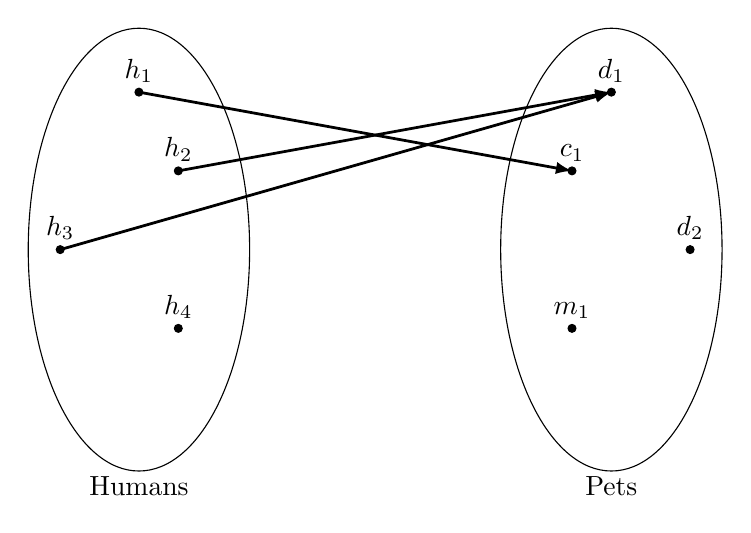
\begin{tikzpicture}
            \draw(2,0) ellipse (40pt and 80pt);
            \draw node at (2,-3){Humans};
            \draw(8,0) ellipse (40pt and 80pt);
            \draw node at (8,-3){Pets};

            %Nodes
            \filldraw (2,2) circle (0.05cm) node[anchor=south]{$h_1$};
            \filldraw (2.5,1) circle (0.05cm) node[anchor=south]{$h_2$};
            \filldraw (1,0) circle (0.05cm) node[anchor=south]{$h_3$};
            \filldraw (2.5,-1) circle (0.05cm) node[anchor=south]{$h_4$};
            \filldraw (8,2) circle (0.05cm) node[anchor=south]{$d_1$};
            \filldraw (7.5,1) circle (0.05cm) node[anchor=south]{$c_1$};
            \filldraw (9,0) circle (0.05cm) node[anchor=south]{$d_2$};
            \filldraw (7.5,-1) circle (0.05cm) node[anchor=south]{$m_1$};

            %Lines
            \draw[->, >=latex, line width=1pt] (2,2) -- (7.5,1);
            \draw[->, >=latex, line width=1pt] (2.5,1) -- (8,2);
            \draw[->, >=latex, line width=1pt] (1,0) -- (8,2);
        \end{tikzpicture}
    \end{center}
    This defines ordered pairs with the human as the first entry, e.g. $(h_1, c_1)$ means that Human 1 owns Cat 1.
\end{exmpl}

This example gives a good intuitive understanding of what a relation is, but it doesn't count as a formal definition of a relation between two sets. We can define a relation as below

\begin{dfn}[label={def:relation2sets}]{Relation Between Two Sets}{dfnrelation2sets}
    A \emph{relation}, $R$, between the sets $A$ and $B$ is a subset of $A \times B$.
    $$R = \{(a,b) | (a,b) \in A \times B\}$$
\end{dfn}

We will look more closely at relations in the future, but for now this should give you a good foundational understanding of sets, how they can relate to each other, and how those relations can create sets themselves.

Next, we will be looking at how sets and functions are related.
% \chapter{Functions}
Now that we have a good unserstanding of sets, relations, Cartesian products, and ordered pairs, let's take a look back at something familiar and reinvestigate functions and see if we can re-cast it in our new language of sets.

\section{The Intuitive Idea of a Function}
Let's take a look at a very familiar function, $f(x) = x^2$

\begin{figure}[ht]
    \centering
    \begin{tikzpicture}
        \begin{axis}[
                xmin=-2,
                xmax=2,
                ymin=-2,
                ymax=3,
                axis lines = middle,
                xlabel=$x$,
                ylabel=$y$,
                clip=false
            ]
            \addplot[samples=25, domain=-1.5:1.5]{x^2} node[right,pos=0.9]{$f(x) = x^2$};
        \end{axis}
    \end{tikzpicture}
    \label{fig:xSquared}
    \caption{Graph of $f(x) = x^2$}
\end{figure}

You can think of this function $f(x)$ as taking some input $x$, and then outputting another value which is the plotted on then axis above. In other words, $f(x)$ takes some value $x \in \R$ and outputs some value $(x,y) \in \R \times \R$, an ordered pair.

There are two criteria necessary in order for a function to be valid, which we have defined below.

\begin{dfn}[label={def:functionClassic}]{Classic Definition of a Function}{dfnfunctionClassic}
    For $f(x)$ to be a valid function it must satisfy the following:
    \begin{itemize}
        \item For every input $x$ in the domain (all the input values) of the function $f$, $f(x)$ must exist (i.e. all inputs give an output)
        \item For every input $x$ in the domain of the function $f$, $f(x)$ must be unique (i.e. no single input can give more than one output)
    \end{itemize}
\end{dfn}

\section{Formal Definition of a Function}

Now let's take a look at creating a formal definition for a function. We already alluded to the core idea that will form the foundation of our definition - when we mentioned that the output of a function is an ordered pair. In fact, we're going to define functions as a set of ordered pairs which follows a few constraints.

\begin{dfn}[label={def:function}]{Function}{dfnFunction}
    A \emph{function} $F$ between the sets $A$ and $B$ is a relation between $A$ and $B$ such that:
    \begin{enumerate}
        \item For every element $x \in A$ there is an element $y \in B$ such that $(x,y) \in F$. This means that for every input $x$, there is some output $y$. This could be written as $F(x) = y$.
        \item If $(x,y) \in F$ and $(x,z) \in F$, then $y = z$. This means that for every input $x$, there must only ever be one output.
    \end{enumerate}
\end{dfn}

Let's take a look at an example of a relation and see if it fits our definition of a function.

\begin{exmpl}[label={exmpl:circleRelation}]{Circle Relation}{xmplcircleRelation}
    Consider the relation $C$ where $(x,y) \in C$ if $x^2 + y^2 = 1$. Is this a function?\\

    First of all, let's plot this relation on a graph, and you'll see why it is called the circle relation:
    \begin{center}
        \begin{tikzpicture}
            \begin{axis}[
                    axis lines=middle,
                    xmin=-2,
                    xmax=2,
                    ymin=-2,
                    ymax=2,
                    axis equal image,
                    clip=false
                ]
                \draw (axis cs:0,0) circle [radius=1];
                \node[label={$x^2 + y^2 = 1$}, anchor=south west] at (axis cs: 1.5,0.5){};
            \end{axis}
        \end{tikzpicture}
    \end{center}
    For this relation to be a function it must satisfy both parts of \cref{def:function}. For part 1, we could define out domain (set $A$ in the definition) as just $\{x | -1 \leq x \leq 1\}$, in which case all elements in the domain have an output.\\
    The more interesting situation comes from looking at part 2, lets see if we can call this a function by restricting the input and output sets to both be $[-1,1]$ - that is the set of all points from -1 to 1 inclusive of the endpoints. This relation fails the definition of a function even with this restricted domain, and we can show this as long as we have 1 example of an input that gives two outputs.

    Let's take $x = 0$, this is within our domain so is a valid input for the relation. Now what values of $y$ exist that satisfy this relation with $x = 0$? In this case, both $y = 1$ \textbf{and} $y = -1$ would satisfy the relation, meaning that both $(0,1)$ and $(0,1) \in C$. This contradicts part 2 of our function definition, therefore this isn't a function.
\end{exmpl}

% \chapter{Introduction to Logic}
In this chapter, we're going to be introduced to mathematical logic. Logic, in this context, is a formal approach to understanding reasoning, looing at the \emph{structure} of an argument, rather than its contents, in order to gain a deeper understanding of how mathematics operates.

\section{Logical Statements}
\begin{dfn}[label={def:statements}]{Statements}{dfnstatements}
    A \emph{statement} is a sentence that is either True (T) or False (F). For example:
    \begin{itemize}
        \item p: $5 > 2$ - this is a statement that is true
        \item q: $2 > 5$ - this is a statement that is false
        \item r: $x > 2$ - this isn't a statement, it has no truth-value in the current context. If we knew more about $x$ we might be able to say if this is true or false.
    \end{itemize}
\end{dfn}

In the above definition, we have included $p,q,r$ at the start of each line. This is a short-hand way of refering to statements (ignoring for a moment that $r$ isn't actually a statement). We can define $p$ as the statement $5 > 2$ and then we can use $p$ to refer to this statement going forward.

It is also possible to create new statements from old ones, but to do this we're going to need to define a few more concepts and their notation

\begin{dfn}[label={def:logicNot}]{Negation (\emph{Not} $\lnot$)}{dfnlogicNot}
    The statement $\lnot p$ (read as \emph{not p}) is true if, and only if, $p$ is false. For example if $p: 5 > 2$, then $\lnot p$ is false, since $p$ is true. However if $p:7<3$ then $p$ is false and $\lnot p$ is true.
\end{dfn}

\begin{dfn}[label={def:logicAnd}]{Conjunction (\emph{And} $\land$)}{dfnlogicAnd}
    The statement $p \land q$ (read as \emph{p and q}) is true if, and only if, both $p$ and $q$ are true. For example:
    \begin{itemize}
        \item $p:5 > 2$ is true and $q: 7< 9$ is true, therefore $p \land q$ is true.
        \item $p:5 > 2$ is true but $q: 7< 3$ is false, therefore $p \land q$ is false.
    \end{itemize}
\end{dfn}

\begin{dfn}[label={def:logicOr}]{Disjunction (Or $\lor$)}{dfnlogicOr}
    The statement $p \lor q$ (read as \emph{p or q}) is true if, and only if, at least one of $p$ and $q$ is true. For example:
    \begin{itemize}
        \item $p:5 > 2$ is true and $q: 7< 9$ is true, therefore $p \lor q$ is true.
        \item $p: 7< 3$ is false but $q:5 > 2$ is true , therefore $p \lor q$ is true.
        \item $p:7 < 3$ and $q: 5 < 2$ are both false, therefore $p \lor q$ is false.
    \end{itemize}
\end{dfn}

Using these three logic symbols, we can construct and analyse statements of varying length and complexity. Let's take a look at an example

\begin{exmpl}[label={exmpl:logicGrayShirt}]{Shirts and Shorts}{xmpllogicGrayShirt}
    Let's analyse the statement ``My shirt is gray but my shorts are not". The first step is to identify the smaller statements that make up this larger one, i.e. the statements ``My shirt is gray" and the statement ``my shorts are not".\\

    Let's define $p:$``my shirt is gray" and $q:$``my shorts are gray". We haven't included the ``not" in the second statment on purpose, let's see how this analysis goes having $q$ be the positive statement.\\

    If we want to combine these two statements back to make the orginal statement, but using our new logic symbols instead, we can write this as
    $$ p \land \lnot q$$

    Notice here we have replaced the word ``but" with our symbol for ``and" since the statements  ``My shirt is gray but my shorts are not" and ``My shirt is gray \textbf{and} my shorts are not" mean the same thing.
\end{exmpl}

\section{Truth Tables}
In the above example, we were able to work out what statements were true and which were false relatively quickly, but more complicated statements require a more robust method of working out which statements are true and which aren't. This is where \emph{truth tables} come in.\\

The way truth tables work is, you have a column for each fundamental statement ( such as $p$ or $q$) and a column for each complex statement (such as $p \land q$), and in each row you put whether your fundamental statements are true or false, and then what that means for the complex statements. Let's try and example

\begin{exmpl}[label={exmpl:truthTableNegation}]{Negation ($\lnot$) Truth Table}{xmpltruthTableNegation}
    Let's look at the truth table for $\lnot$, to start we have a column for the statement $p$ and a column for the statement $\lnot p$:
    \begin{center}
        \begin{tabular}{|c|c|}
            \hline
            $p$ & $\lnot p$ \\
            \hline
        \end{tabular}
    \end{center}
    Now we need to add in our rows, since $p$ can be either true or false, we will need 2 rows:
    \begin{center}
        \begin{tabular}{|c|c|}
            \hline
            $p$ & $\lnot p$ \\
            \hline
            T   &           \\
            \hline
            F   &           \\
            \hline
        \end{tabular}
    \end{center}
    Now we fill in our $\lnot p$ column based off of the $p$ column, remembering that $\lnot p$ is false if $p$ is true:
    \begin{center}
        \begin{tabular}{|c|c|}
            \hline
            $p$ & $\lnot p$ \\
            \hline
            T   & F         \\
            \hline
            F   & T         \\
            \hline
        \end{tabular}
    \end{center}
\end{exmpl}

Let's take a look at another example, this time we'll look at conjunction, i.e. a statement like $p \land q$.

\begin{exmpl}[label={exmpl:truthTableConjunction}]{Conjunction ($\land$) Truth Table}{xmpltruthTableConjunction}
    In this example, we now have 2 fundamental statements, $p$ and $q$. Let's start a table which includes both of these, and the statement $p \land q$:
    \begin{center}
        \begin{tabular}{|c|c|c|}
            \hline
            $p$ & $q$ & $p \land q$ \\
            \hline
        \end{tabular}
    \end{center}
    Both of these fundamental statements could be either true or false, which gives us 4 possible configurations, as shown in the table below
    \begin{center}
        \begin{tabular}{|c|c|c|}
            \hline
            $p$ & $q$ & $p \land q$ \\
            \hline
            T   & T   &             \\
            \hline
            T   & F   &             \\
            \hline
            F   & T   &             \\
            \hline
            F   & F   &             \\
            \hline
        \end{tabular}
    \end{center}
    \vspace{0.5cm}
    Now we can use our definition for conjunction, \cref{def:logicAnd}, to fill in the rest of the table:
    \begin{center}
        \begin{tabular}{|c|c|c|}
            \hline
            $p$ & $q$ & $p \land q$ \\
            \hline
            T   & T   & T           \\
            \hline
            T   & F   & F           \\
            \hline
            F   & T   & F           \\
            \hline
            F   & F   & F           \\
            \hline
        \end{tabular}
    \end{center}
    \vspace{0.5cm}
    Since $\land$ requires both inputs to be true, the truth table for conjunction returns false in all other instances
\end{exmpl}

Lets also look at the truth table for disjunction, i.e. statements like $p \lor q$.

\begin{exmpl}[label={exmpl:truthTableDisjunction}]{Disjunction ($\lor$) Truth Table}{xmpltruthTableDisjunction}
    Similarly to \cref{exmpl:truthTableConjunction}, we have 2 fundamental statements, $p$ and $q$. Let's start a table which includes both of these, and the statement $p \lor q$, and fill in the truth values for the fundamental statements:
    \begin{center}
        \begin{tabular}{|c|c|c|}
            \hline
            $p$ & $q$ & $p \lor q$ \\
            \hline
            T   & T   &            \\
            \hline
            T   & F   &            \\
            \hline
            F   & T   &            \\
            \hline
            F   & F   &            \\
            \hline
        \end{tabular}
    \end{center}
    \vspace{0.5cm}
    Now we can use our definition for disjunction, \cref{def:logicOr}, to fill in the rest of the table: \begin{center}
        \begin{tabular}{|c|c|c|}
            \hline
            $p$ & $q$ & $p \lor q$ \\
            \hline
            T   & T   & T          \\
            \hline
            T   & F   & T          \\
            \hline
            F   & T   & T          \\
            \hline
            F   & F   & F          \\
            \hline
        \end{tabular}
    \end{center}
    \vspace{0.5cm}
    Since $\lor$ only requires one input to be true, the truth table for disjunction returns true in all instances except where both inputs are false.
\end{exmpl}

Now let's look at one final example, the truth table for the statement $\lnot p \lor \lnot q$
\newpage

\begin{exmpl}[label={exmpl:truthTableNPOQ}]{$\lnot p \lor \lnot q$ Truth Table}{xmpltruthTableNPOQ}
    Lets start by adding in all the table headers we're going to need and the truth value for out fundamental statements. In this example we have our two fundamental statements, $p$ and $q$, but we also have the statements $\lnot p$ and $\lnot q$, and then finally we have $\lnot p \lor \lnot q$:
    \begin{center}
        \begin{tabular}{|c|c|c|c|c|}
            \hline
            $p$ & $q$ & $\lnot p$ & $\lnot q$ & $\lnot p \lor \lnot q$ \\
            \hline
            T   & T   &           &           &                        \\
            \hline
            T   & F   &           &           &                        \\
            \hline
            F   & T   &           &           &                        \\
            \hline
            T   & F   &           &           &                        \\
            \hline
        \end{tabular}
    \end{center}
    \vspace{0.5cm}
    Now let's first handle the two negation columns and fill those in based on our negation table, \cref{exmpl:truthTableNegation}
    \begin{center}
        \begin{tabular}{|c|c|c|c|c|}
            \hline
            $p$ & $q$ & $\lnot p$ & $\lnot q$ & $\lnot p \lor \lnot q$ \\
            \hline
            T   & T   & F         & F         &                        \\
            \hline
            T   & F   & F         & T         &                        \\
            \hline
            F   & T   & T         & F         &                        \\
            \hline
            F   & F   & T         & T         &                        \\
            \hline
        \end{tabular}
    \end{center}
    \vspace{0.5cm}

    Finally, let's use the values of $\lnot p$ and $\lnot q$ as the inputs for our disjunction table, \cref{exmpl:truthTableDisjunction}, giving our final output:

    \begin{center}
        \begin{tabular}{|c|c|c|c|c|}
            \hline
            $p$ & $q$ & $\lnot p$ & $\lnot q$ & $\lnot p \lor \lnot q$ \\
            \hline
            T   & T   & F         & F         & F                      \\
            \hline
            T   & F   & F         & T         & T                      \\
            \hline
            F   & T   & T         & F         & T                      \\
            \hline
            F   & F   & T         & T         & T                      \\
            \hline
        \end{tabular}
    \end{center}
    \vspace{0.5cm}

    Notice anything about this final column? It is the exact opposite (the \emph{negation}) of our conjunction ($\land$) table:
    \begin{center}
        \begin{tabular}{|c|c|c|c|}
            \hline
            $p$ & $q$ & $p \land q$ & $\lnot(p \land q)$ \\
            \hline
            T   & T   & T           & F                  \\
            \hline
            T   & F   & F           & T                  \\
            \hline
            F   & T   & F           & T                  \\
            \hline
            F   & F   & F           & T                  \\
            \hline
        \end{tabular}
    \end{center}
    \vspace{0.5cm}
    This shows that $\lnot (p \land q)$ is \emph{logically equivalent} to $\lnot p \lor \lnot q$.
\end{exmpl}

\section{Logical Equivalence of Two Statements}
In the previous example, we introduced the idea of \emph{logical equivalence}, the idea of two different statements being the same thing written in two different ways.

\begin{dfn}[label={def:logicalEquivalence}]{Logical Equivalence}{dfnlogicEquiv}
    Two statements, $p$ and $q$ are \emph{logically equivalent} if they have the same truth table. This is written as $$ p \equiv q$$
\end{dfn}

Let's look at a simple example to understand what this means

\begin{exmpl}[label={exmpl:logicEquivNotNot}]{Double Negative}{dfnlogicEquivNotNot}
    Let's say we have the statement $p$, what can we say about the statement $\lnot (\lnot p)$? Intuitively, we know that a double negative cancels out, for example saying ``I'm not not hungry" is the same as saying ``I \textbf{am} hungry", but can we verify this using truth tables?

    First let's build our truth table with the fundamental statement values filled in:
    \begin{center}
        \begin{tabular}{|c|c|c|}
            \hline
            $p$ & $\lnot p$ & $\lnot (\lnot p)$ \\
            \hline
            T   &           &                   \\
            \hline
            F   &           &                   \\
            \hline
        \end{tabular}
    \end{center}
    \vspace{0.5cm}
    Now lets fill in our $\lnot p$ column:
    \begin{center}
        \begin{tabular}{|c|c|c|}
            \hline
            $p$ & $\lnot p$ & $\lnot (\lnot p)$ \\
            \hline
            T   & F         &                   \\
            \hline
            F   & T         &                   \\
            \hline
        \end{tabular}
    \end{center}
    \vspace{0.5cm}
    Finally lets fill in our $\lnot (\lnot p)$ column:
    \begin{center}
        \begin{tabular}{|c|c|c|}
            \hline
            $p$ & $\lnot p$ & $\lnot (\lnot p)$ \\
            \hline
            T   & F         & T                 \\
            \hline
            F   & T         & F                 \\
            \hline
        \end{tabular}
    \end{center}
    \vspace{0.5cm}
    The columns for $p$ and $\lnot(\lnot p)$ are indentical, therefore they are logically equivalent, $p \equiv \lnot(\lnot p)$.
\end{exmpl}

\section{Tautologies and Contradictions}
There is a special kind of statement known as a \emph{tautology} which we'll define as follows

\begin{dfn}[label={def:tautology}]{Tautology}{dfnTautology}
    A \emph{tautology, t,} is a statement which is always true.
\end{dfn}

Let's look at an example of a truth table when we use a tautology

\begin{exmpl}[label={exmpl:tautologyOr}]{Tautology $t \lor p$}{xmpltautologyOr}
    Let's say we have some tautology $t$ and some statement $p$ and we want to analyse $t \lor p$. The truth table will be as follows
    \begin{center}
        \begin{tabular}{|c|c|c|}
            \hline
            $t$ & $p$ & $t \lor p$ \\
            \hline
            T   & T   & T          \\
            \hline
            T   & F   & T          \\
            \hline
        \end{tabular}
    \end{center}
    \vspace{0.5cm}
    So using or ($\lor$) with a tautology gives another tautology.
\end{exmpl}

There is another special kind of logical statement, known as a \emph{contradiction}, which we define as follows

\begin{dfn}[label={def:contradiction}]{Contradiction}{dfnContradiction}
    A \emph{contradiction, c,} is a statement which is always false.
\end{dfn}

Let's look at an example of a truth table when we use a contradiction

\begin{exmpl}[label={exmpl:contradictionAnd}]{Contradiction $c \land p$}{xmplcontradictionAnd}
    Let's say we have some contradiction $c$ and some statement $p$ and we want to analyse $c \land p$. The truth table will be as follows
    \begin{center}
        \begin{tabular}{|c|c|c|}
            \hline
            $c$ & $p$ & $c \land p$ \\
            \hline
            F   & T   & F           \\
            \hline
            F   & F   & F           \\
            \hline
        \end{tabular}
    \end{center}
    \vspace{0.5cm}
    So using and ($\land$) with a contradiction gives another contradiction.
\end{exmpl}

\section{3 Ways to Show Logical Equivalence}
\label{sec:logicalEquivalence}

Let's take a look at 3 different ways to argue that two complex statements are logically equivalent.

Let's say we want to determine if $$\lnot (p \lor q) \equiv \lnot p \land \lnot q$$

\begin{enumerate}
    \item \textbf{Reason check with examples}: The first method to check if two statements are equivalent is to try making real world examples. Let's set $p$: Chocolate is sour and $q$: Chocolate is savory. Putting these into the left hand side we get
          $$\textit{It is \emph{NOT} the case that chocolate is either sour OR savory }$$
          Looking at the right hand side we get
          $$\textit{Chocolate is \emph{NOT} sour and it is \emph{NOT} savory }$$
          Read these two statements over a few times and we notice that they are, in fact, saying the same thing - chocolate is neither sour nor savory.
    \item \textbf{Truth Tables}: A more formal way to check if two statements are equivalent is to use truth tables. Here are the truth tables for the above statements:
          \begin{center}
              \begin{tabular}{|c|c|c|c|c|c|c|}
                  \hline
                  $p$ & $q$ & $\lnot p$ & $\lnot q$ & $p \lor q$ & $\lnot (p \lor q)$ & $\lnot p \land \lnot q$ \\
                  \hline
                  T   & T   & F         & F         & T          & F                  & F                       \\
                  \hline
                  T   & F   & F         & T         & T          & F                  & F                       \\
                  \hline
                  F   & T   & T         & F         & T          & F                  & F                       \\
                  \hline
                  F   & F   & T         & T         & F          & T                  & T                       \\
                  \hline
              \end{tabular}
          \end{center}
          This formally proves these two statements are equivalent.
    \item \textbf{Logical Laws}: The final way to determining if statements are logically equivalent is to use logical laws, some of which we have already seen, like the examples listed below:
          \begin{itemize}
              \item DeMorgan's Laws:
                    $$\lnot(p \lor q) \equiv \lnot p \land \lnot q$$
                    $$\lnot(p \land q) \equiv \lnot p \lor \lnot q$$
              \item Double Negative:
                    $$p \equiv \lnot(\lnot p)$$
              \item Identity Laws:
                    $$p \lor c \equiv p$$
                    $$p \land t \equiv p$$
              \item Universal Bound laws:
                    $$p \land c \equiv c$$
                    $$p \lor t \equiv t$$
          \end{itemize}
          All of the above can be shown to be true using truth tables and they come in very handy when evaluating complex statements.
          \begin{exmpl}[label={exmpl:logicLaws}]{Using logical laws}{xmpllogicLaws}
              Let's use the laws defined above to evaluate $$ (\lnot (p \lor \lnot q)) \land t$$
              First of all, we can use the indetity law with tautologies to say that
              $$ (\lnot (p \lor \lnot q)) \land t \equiv  \lnot (p \lor \lnot q)$$
              We can then use the first of DeMorgan's laws to say
              $$\lnot (p \lor \lnot q) \equiv \lnot p \land \lnot (\lnot q)$$
              and finally we can use the Double Negative law to say
              $$ \lnot p \land \lnot (\lnot q) \equiv \lnot p \land q$$
              so we have that
              $$ (\lnot (p \lor \lnot q)) \land t \equiv \lnot p \land q$$
          \end{exmpl}
\end{enumerate}

\section{Conditional Statements}
Now that we have a good understanding of statements and logical analysis, let's take a look at \emph{conditional statements}.

\begin{dfn}[label={def:conditionalStatements}]{Conditional Statements}{dfnConditionalStatements}
    A \emph{conditional statement} is a statement of the form ``if $p$ is true, then $q$ is true" where $p$ is called the \emph{hypothesis} and $q$ is called the \emph{conclusion}. This is written as $$p \to q$$
\end{dfn}

Let's see how we can combine this with our current understanding of logic by seeing if we can create a truth table

\newpage
\begin{exmpl}[label={exmpl:truthTableConditional}]{Conditional Statement Truth Table}{xmpltruthTableConditional}
    Let's start by creating the outline of our table and filling in the possible values for our two statements
    \begin{center}
        \begin{tabular}{|c|c|c|}
            \hline
            $p$ & $q$ & $p \to q$ \\
            \hline
            T   & T   &           \\
            \hline
            T   & F   &           \\
            \hline
            F   & T   &           \\
            \hline
            F   & F   &           \\
            \hline
        \end{tabular}
    \end{center}
    \vspace{0.5cm}

    Now how do we fill in the final column? \Cref{def:conditionalStatements} says that if $p$ is true, then $q$ must be true, therefore the statement is true in the first row since both $p$ and $q$ are true.\\

    In the second row, $p$ is still true but $q$ is false, meaning that $p$ being true does not then lead to $q$ being true, so our conditional statement is false.\\

    For the final two rows, our hypothesis $p$ is false, but our definition of a conditional statement starts with ``if $p$ is true" so the conditional statement doesn't actually apply here. In this case we would say they are \emph{vacuously true}, meaning that we can't properly evaluate the statement in this case, so we can neither prove nor disprove it. In this case we give the row in the truth table the value of true (T) so our final truth table for a conditonal statement is

    \begin{center}
        \begin{tabular}{|c|c|c|}
            \hline
            $p$ & $q$ & $p \to q$ \\
            \hline
            T   & T   & T         \\
            \hline
            T   & F   & F         \\
            \hline
            F   & T   & T         \\
            \hline
            F   & F   & T         \\
            \hline
        \end{tabular}
    \end{center}
    \vspace{0.5cm}
    Let's add two new columns to the table to better explain this
    \begin{center}
        \begin{tabular}{|c|c|c|c|c|}
            \hline
            $p$ & $q$ & $p \to q$ & $\lnot p$ & $\lnot p \lor q$ \\
            \hline
            T   & T   & T         & F         & T                \\
            \hline
            T   & F   & F         & F         & F                \\
            \hline
            F   & T   & T         & T         & T                \\
            \hline
            F   & F   & T         & T         & T                \\
            \hline
        \end{tabular}
    \end{center}
    \vspace{0.5cm}
    These extra two columns give a better understanding of why the two bottom rows of our original table evaluate to true. The last column is another way of phrasing our conditional statement. Rather than saying ``if $p$ is true, then $q$ is true" what we're saying is ``either $p$ is false, or $p$ is true". Take a moment to re-read this and convince yourself these are the same thing.\\

    Consider the statement ``if I study hard, then I will pass". We can say that $p$: ``I study hard" and $q$:``I will pass". Using these we can rewrite the previous statement as
    $$p \to q$$
    Now let's consider the statement ``Either I don't study hard, or I pass". Using the same fundamental statements as above, we can write this as
    $$\lnot p \lor q$$
\end{exmpl}

\newpage

\section{Vacuously True Statements}
As we have discussed above, when the hypothesis of a conditional statement is false, we say the statement is \emph{vacuously true} - i.e. true in a way that is unimportant and doesn't tell us anything.\\

For example, take the following statement\\
\begin{center}
    If the sky is purple, then grass is green
\end{center}
This is of the form \emph{if $p$ then $q$}. As we demonstrated above, we can rewrite any statement of the form $p \to q$ to the form $\lnot p \lor q$ so let's do that here
\begin{center}
    Either the sky is not purple or grass is green
\end{center}
This second form makes it much easier to see that the conditional statement is true since grass is (usually) green, meaning the statement is true regardless of whether the sky is purple or not.

\section{Negating a Conditional Statement}
\label{sec:negatingConditional}
Let's take a look at what it means to negate a conditional statement, that is to evaluate a statement such as
$$\lnot (p \to q)$$
From our examples above, we know that this is equivalent to using a disjunctive argument. That is
$$\lnot (p \to q) \equiv \lnot (\lnot p \lor q)$$
Now we can use DeMorgan's law (stated in \Cref{sec:logicalEquivalence} ) to rewrite this as
\begin{align*}
    \lnot (p \to q) & \equiv \lnot (\lnot p \lor q)                            \\
                    & \equiv \lnot \lnot p \land \lnot q \tag*{DeMorgan's Law} \\
                    & \equiv p \land \lnot q \tag*{Double Negation}
\end{align*}
This should make sense if we remember what a conditional statement is saying. The statement $p \to q$ is saying that if $p$ is true, then $q$ must be true, so the negation of this would be if $p$ is true, then $q$ must be false. In other words $\lnot (p \to q)$ is only true when $p$ is true \emph{and} $q$ is false. This can be seen in the truth table we used before:

\begin{center}
    \begin{tabular}{|c|c|c|c|}
        \hline
        $p$ & $q$ & $p \to q$ & $\lnot (p \to q)$ \\
        \hline
        T   & T   & T         & F                 \\
        \hline
        T   & F   & F         & T                 \\
        \hline
        F   & T   & T         & F                 \\
        \hline
        F   & F   & T         & F                 \\
        \hline
    \end{tabular}
\end{center}

\section{Contrapositive of a Conditional Statement}
There are a few other types of statements that are all related to the conditional statement, in this section we're going to evaluate the \emph{contrapositive} statement.

\begin{dfn}[label={def:contrapositive}]{Contrapositive Statements}{dfncontrapositive}
    For a conditional statement $p \to q$, the \emph{contrapositive} statement is $$\lnot q \to \lnot p$$ These two statements are logically equivalent
\end{dfn}

We can demonstrate this using the truth table below
\begin{center}
    \begin{tabular}{|c|c|c|c|c|c|}
        \hline
        $p$ & $q$ & $\lnot p$ & $\lnot q$ & $p \to q$                          & $\lnot q \to \lnot p$              \\
        \hline
        T   & T   & F         & F         & T                                  & T (Vacuously)                      \\
        \hline
        T   & F   & F         & T         & F (\cref{sec:negatingConditional}) & F (\cref{sec:negatingConditional}) \\
        \hline
        F   & T   & T         & F         & T (Vacuously)                      & T (Vacuously)                      \\
        \hline
        F   & F   & T         & T         & T (Vacuously)                      & T                                  \\
        \hline
    \end{tabular}
\end{center}

We can also say that, since we know $p \to q \equiv \lnot p \lor q$ we can do the same with $\lnot q \to \lnot p$ and get
\begin{align*}
    \lnot q \to \lnot p & \equiv \lnot (\lnot q) \lor \lnot p          \\
                        & \equiv q \lor \lnot p \tag*{Double Negation} \\
                        & \equiv \lnot p \lor q
\end{align*}
Therefore $p \to q \equiv \lnot q \to \lnot p$.\\

We can demonstrate this using the example we used previously of $p$: ``I study hard" and $p$:``I will pass". Here we have $p \to q$ is the statement ``If I study hard, then I will pass" and $\lnot q \to \lnot p$ can be interpreted as ``If I don't pass, then I didn't study hard".\\

Notice that at no point in this example did we come across the statement ``If I pass, then I studied hard". This would be the conditional statement $q \to p$. This is something to be carful of when tackling mathematical logic, something that may seem equivalent when spoken in English isn't necessarily equivalent from a logical perspective.

\section{Converse and Inverse of Conditional Statements}

\begin{dfn}[label={def:conditionalConverse}]{Converse of a Conditional Statememt}{dfnConditionalConverse}
    The \emph{converse} of a conditional statement $p \to q$ is the statement $q \to p$. It is important to note that
    $$p \to q \not \equiv q \to p$$
\end{dfn}

Let's look at an example to fully understand this distinction

\begin{exmpl}[label={exmpl:conditionalConverse}]{Converse of a Conditional Statement}{xmplConditionalConverse}
    Let's take the statement ``If it's a dog, then it's a mammal". In this example $p$: ``It is a dog" and $q$: ``It is a mammal". In this case $p \to q$ is true since the definition of a dog requires it to be a mammal - there a no non-mammal dogs.\\

    If we consider the converse $q \to p$, this would be ``If it is a mammal, then it is a dog". This is not the same thing, there are a lot of examples of non-dog mammals.
\end{exmpl}

\begin{dfn}[label={def:conditionalInverse}]{Inverse of a Conditional Statememt}{dfnConditionalInverse}
    The \emph{inverse} of a conditional statement $p \to q$ is the statement $\lnot p \to \lnot q$. This is in effect the converse of the contrapositive of $p \to q$ and as such
    $$p \to q \not \equiv \lnot p \to \lnot q$$
    but
    $$\lnot p \to \lnot q \equiv q \to p$$
    That is to say, the inverse and the converse are logically equivalent.
\end{dfn}

\begin{exmpl}[label={exmpl:conditionalInverse}]{Inverse of a Conditional Statement}{xmplConditionalInverse}
    Let's take a look at the inverse using the same example as above. If $p$: ``It is a dog" and $q$: ``It is a mammal", then the inverse $\lnot p \to \lnot q$ would be ``If it is not a dog, then it is not a mammal". Again, this is false since there a a lot of examples on mammals that are not dogs.
\end{exmpl}

\section{Biconditional Statements}
We have seen above that a statement and its converse are not logically equivalent, that doesn't, however, mean they can't both be true. This gives us a \emph{biconditional} statement.

\begin{dfn}[label={def:biconditional}]{Biconditional Statement}{dfnBiconditional}
    A \emph{biconditional statement} $p \iff q$ is a statement such that $p \to q$ is true, and $q \to p$ is also true. This is usually read as \begin{center}
        $p$ is true \emph{if and only if} $q$ is true
    \end{center}
\end{dfn}

Let's take a look at an example

\begin{exmpl}[label={exmpl:biconditional}]{Biconditional Statement}{xmplBiconditional}
    Let's use an example from earlier ``If I study hard, then I will pass". This is the statement $p \to q$. The statement $q \to p$ would be ``If I pass, then I studied hard". Both of these statements can be true at the same time, so we can say ``I will pass if and only i, I study hard", this is the statement $p \iff q$.\\

    We can also write this as ``If I study hard, then I will pass \textbf{AND} if I pass, then I studied hard". This ``and" indicates we could write this statement in the following way
    $$ (\lnot p \lor q ) \land (\lnot q \lor p)$$
\end{exmpl}
% \chapter{Logical Arguments}
\label{chap:logicalArguments}
\section{Introduction to Logical Arguments}
In logic, \emph{arguments} are a list of statements (called \emph{premises}) followed by a conclusion, usually of the form ``If $p$ and $q$, then $r$".

\begin{dfn}[label={def:validArguments}]{Valid Arguments}{dfnValidArguments}
    A \emph{valid argument} is an argument where the conclusion logically follows from the premises, regardless of the truth value of the premises.
\end{dfn}

\begin{exmpl}[label={exmpl:validArgument}]{A Valid Argument}{xmplValidArgument}
    Let's take a look at the form a valid argument would take. Our two premises are
    \begin{center}
        If I do the dishes, I will feel better\\
        I do the dishes
    \end{center}
    Our conclusion therefore is
    \begin{center}
        I feel better
    \end{center}
    This argument is \emph{valid} because, if our two premises are true, then the conclusion logically follows
\end{exmpl}

\begin{exmpl}[label={exmpl:invalidArgument}]{An Invalid Argument}{xmplInvalidArgument}
    Let's take a look what an \emph{invalid} argument would look like. Our premises are the same as before
    \begin{center}
        If I do the dishes, I will feel better\\
        I do the dishes
    \end{center}
    This time our conclusion is
    \begin{center}
        The sky is blue
    \end{center}
    In this case, the conclusion does not follow from the premises, nothing about us doing the dishes indicates that the sky is blue.

    Note that it doesn't matter if the conclusion is true or not, the argument is invalid because it conclusion doesn't follow from the premises.
\end{exmpl}

This particluar form of argument actually has a name

\begin{dfn}[label={def:modusPonens}]{Modus Ponens Argument}{dfnModusPonens}
    A \emph{Modus Ponens} argument is an argument of the form
    \begin{center}
        If $p$, then $q$.\\
        $p$.\\
        Therefore, $q$.
    \end{center}
\end{dfn}

Let's use a truth table to try and get a better appreciation for this style of argument

\begin{center}
    \begin{tabular}{|c|c|c|c|c|}
        \hline
        \multicolumn{2}{|c|}{Variables} & \multicolumn{2}{|c|}{Premises} & Conclusion             \\
        \hline
        $p$                             & $q$                            & $p \to q$  & $p$ & $q$ \\
        \hline
        T                               & T                              & T          & T   & T   \\
        \hline
        T                               & F                              & F          & T   & N.A \\
        \hline
        F                               & T                              & T          & F   & N.A \\
        \hline
        F                               & F                              & T          & F   & N.A \\
        \hline
    \end{tabular}
\end{center}

We have put ``N.A" in the final 3 rows of the last column for one very important reason - our argument is assuming that both premises are true and this only occurs in the top row so this is the only one we care about evaluating.\\

Another important form of a logical argument is essentially the contrapositive (\cref{def:contrapositive}) of the Modus Ponens argument

\begin{dfn}[label={def:modusTollens}]{Modus Tollens Argument}{dfnModusTollens}
    A \emph{Modus Tollens} argument is an argument of the form
    \begin{center}
        If $p$, then $q$.\\
        $\lnot q$.\\
        Therefore, $\lnot p$.
    \end{center}
\end{dfn}

Let's take a look at the truth table for this style of argument as well
\begin{center}
    \begin{tabular}{|c|c|c|c|c|}
        \hline
        \multicolumn{2}{|c|}{Variables} & \multicolumn{2}{|c|}{Premises} & Conclusion                         \\
        \hline
        $p$                             & $q$                            & $p \to q$  & $\lnot q$ & $\lnot p$ \\
        \hline
        T                               & T                              & T          & F         & N.A       \\
        \hline
        T                               & F                              & F          & T         & N.A       \\
        \hline
        F                               & T                              & T          & F         & N.A       \\
        \hline
        F                               & F                              & T          & T         & T         \\
        \hline
    \end{tabular}
\end{center}

Similarly to before, we only want to evaluate when both of our premises are true, in this case that is the final row. When both our premises are true, $p$ is false and therefore our conclusion, $\lnot p$ is true, as required.

Let's look at an example of a Modus Tollens argument

\begin{exmpl}[label={exmpl:modusTollens}]{Modus Tollens Argument}{xmplModusTollens}
    Let's evaluate the following argument
    \begin{center}
        If I am the POTUS then I'm an American citizen.\\
        I am not an American citizen.\\
        Therefore, I am not the POTUS.
    \end{center}
    Here we have $p$:``I am the POTUS" and $q$:``I'm an American citizen". This is an argument of the form
    $$p \to q$$
    $$\lnot q$$
    $$\text{therefore } \lnot p$$
\end{exmpl}

\begin{dfn}[label={def:generalization}]{Generalization}{dfnGeneralization}
    A \emph{generalization} is an argument of the form
    $$p.$$
    $$\text{Therefore } p \lor q.$$
\end{dfn}

\begin{exmpl}[label={exmpl:generalization}]{Generalization}{xmplGeneralization}
    An example of a \emph{generalization} is
    \begin{center}
        The sky is blue.\\
        Therefore, the sky is blue or grass is purple
    \end{center}
    Since the sky is blue, our conclusion here is true. It doesn't matter if grass is purple or not.
\end{exmpl}
\vspace{1cm}

The opposite of a generalization is called \emph{specialization}.

\begin{dfn}[label={def:specialization}]{Specialization}{dfnSpecialization}
    A \emph{specialization} is an argument of the form
    $$p \land q$$
    $$\text{Therefore } p$$
\end{dfn}

\begin{exmpl}[label={exmpl:specialization}]{Specialization}{xmplSpecialization}
    An example of a \emph{specialization} is
    \begin{center}
        The sky is blue and grass is green.\\
        Therefore, the sky is blue.
    \end{center}
    Since both of the conditions in our premis are true, then we can pull one of them out and say that is definitely true.
\end{exmpl}
\newpage

One final, but very important, form of an argument is a \emph{contradiction}, not to be confused with \Cref{def:contradiction}.

\begin{dfn}[label={def:contradictionArgument}]{Contradiction (Argument)}{dfnContradictionArgument}
    A \emph{contradiction} is an argument of the form
    $$\lnot p \to c$$
    $$\text{Therefore } p$$
    Where $c$ is the contradiction from \cref{def:contradiction}. In plain English this argument says ``Assume $p$ is false, this leads to a contradiction. Therefore $p$ must be true".
\end{dfn}
\vspace{1cm}
We shall look at an example of this later on.

\section{Analyzing an Argument for Validity}
Let's take a look at an argument and try analyzing it to see if the argument is valid.

\begin{exmpl}[label={exmpl:argumentValidity}]{Analysing an Argument for Validity}{xmplArgumentValidity}
    Let's look at the following argument\\
    \begin{center}
        If I'm skilled at poker, then I will win.\\

        I won money playing poker.\\

        Therefore, I'm skilled at poker
    \end{center}
    The first premise is of the form $p \to q$ where $p$: \emph{I'm skilled at poker} and $q$:\emph{I will win}.

    Using these statements, the full format of the argument is \\
    \begin{center}
        $p \to q$\\
        $q$\\
        Therefore $p$
    \end{center}

    This is not a valid argument form. There could be other reasons I won money at poker other than being skilled - it could have just been pure luck, or the other players may have been even worse at poker.\\

    This argument would be valid if the first premise instead was ``\emph{If I win, then I am skilled at poker}".
\end{exmpl}

\chapter{Predicates and Quantified Statements}

\section{Predicates and their Truth Sets}
Recall previously we defined a statement as something that could be eaither \emph{true} or \emph{false} (\cref{def:statements}). This is obvious for statements such as $7 > 5$ or $3 > 5$ - these are true and false respectively.

How do we evaluate the truth value of a statement containing a variable, such as $x > 5$? This doesn't fit out definition of a statement since its truth value is dependant on tha value of $x$ - we call this a \emph{predicate}

\begin{dfn}[label={def:predicate}]{Predicate}{dfnPredicate}
    A \emph{predicate} is a sentence depending on variables which becomes a statement upon substituting values in the domain.
\end{dfn}

Let's look at en example to get a better idea of what this definition is saying

\begin{exmpl}[label={exmpl:predicate}]{Predicate}{xmplPredicate}
    Consider the following
    $$P(x): x \text{ is a factor of } 12 \text{ within domain } \Z^+ $$
    In English this says ``$x$ is a positive integer that is a factor of 12''.

    The domain, $\Z^+$ is a key part of a predicate, we need to know what possible values our variable(s) could take in order to evaluate the truth value of the statements when we subtitute them in.

    Let's say that $x = 6$, $6 \in \Z^+$ and $12 \div 6 = 2$. Since $6$ is in out domain and it satisfies the condition of being a factor of 12, we can say that $P(6)$ is \emph{true}.

    If we say $x = 5$, $5 \in \Z^+$ but 5 is not a factor of 12. Since 5 does not satisfy the condition of being a factor of 12, we can say that $P(5)$ is \emph{false}.

    Similarly if we say $x = \frac{1}{3}$, $\frac{1}{3} \notin \Z^+$ therefore $P(\frac{1}{3})$ is \emph{invalid}.
\end{exmpl}
\newpage
\begin{dfn}[label={def:truthSet}]{Truth Set}{dfnTruthSet}
    The \emph{Truth Set} of a predicate $P(x)$ over domain $D$ is
    $$\{x \in D | P(x)\}$$
    i.e. all values $x$ in the domain $D$ where $P(x)$ is true.
\end{dfn}
\begin{exmpl}[label={exmpl:truthSet}]{Truth Set}{xmplTruthSet}
    Using the same example as above
    $$P(x): x \text{ is a factor of } 12 \text{ within domain } \Z^+ $$
    The set of all positive integers that are factors of 12 is
    $$TS=\{1, 2,3,4,6,12 \}$$
    notice we have $TS \subseteq \Z^+$.
\end{exmpl}

\section{Universal and Existential Quantifiers}
We have used a lot of symbols and notation so far in this course, let's now take a look at 2 more symbols that are used in logical arguments, the \emph{universal} and \emph{existential} quantifiers.

\begin{dfn}[label={def:universalQuantifier}]{Universal Quantifier}{dfnUniversalQuantifier}
    The \emph{Universal Quantifier}, $\forall$, is read as ``for all'' and means all elements of a domain that satisfy a condition. E.g. $\forall x \in \R$ means ``for all real numbers''.
\end{dfn}
The main use of this quatifier is, unsurprisingly, to quantify predicates. That is, to state for which values of $x$ it is true. For example,
$$\forall x \in D, P(x)$$
means ``for all values of $x$ in the domain $D$, $P(x)$ is true''. Notice how much quicker it is to write this out using the quantifier.

\begin{exmpl}[label={exmpl:universalQuantifier}]{Universal Quantifier}{xmplUniversalQuantifier}
    Let's see how we can use this quantifier with our example from earlier

    \begin{center}
        Every dog is a mammal
    \end{center}

    The first thing to notice is the use of the word ``every''. If you see this in a written statement, it is the same as using ``for all''.

    Now let's call $D$ the set of all dogs, so for a single dog we would say $x \in D$.

    Finally let's say we have a predicate $P(x)$ such that $P(x): x$ is a mammal.

    Using this we can rewrite the above statement as
    $$\forall x \in D, P(x)$$
\end{exmpl}

Now let's take a look at the other quantifier we mentioned above

\begin{dfn}[label={def:existentialQuantifier}]{Existential Quantifier}{dfnExistentialQuantifier}
    The \emph{Existential Quantifier}, $\exists$, is read as ``there exists'' and means there is at least one element in a domain that satisfies a condition. E.g. $\exists x \in \R$ means ``there exists at least one real number''.
\end{dfn}

Similarly to the universal quantifier, the main use of this quatifier is to quantify predicates. For example,
$$\exists x \in D, P(x)$$
means ``there exists at least one $x$ in the domain $D$ such that $P(x)$ is true''. Let's look at an example.

\begin{exmpl}[label={exmpl:existentialQuantifier}]{Existential Quantifier}{xmplExistentialQuantifier}
    Let's see how we can use this quantifier with the following statement

    \begin{center}
        Some person is the oldest in the world
    \end{center}

    The first thing to notice is the use of the word ``some''. If you see this in a written statement, it is the same as using ``there exists''.

    Now let's call $D$ the set of all people in the world, so for a single person we would say $x \in D$.

    Finally let's say we have a predicate $P(x)$ such that $P(x): x$ is the oldest.

    Using this we can rewrite the above statement as
    $$\exists x \in D, P(x)$$
\end{exmpl}

It is important to remember the difference between a \emph{statement} (\cref{def:statement}) and a \emph{predicate}(\cref{def:predicate}), and the difference in notation:
\begin{itemize}
    \item \textbf{Statement:} $P:$ Spot is a mammal - this is looking at a specific dog, menaing this is either true or false, therefore it is a statements
    \item \textbf{Predicate} $P(x):$ $x$ is a mammal - the truth of this depends on $x$, therefore it is a predicate
    \item \textbf{Quantifier}: $Q:\forall x \in D, P(x):$ Every dog is a mammal - putting a quantifier infront of a predicate turns it into a statement.
\end{itemize}

\section{Negating Universal and Existential Quantifiers}
Consider the following statement
$$P: \forall x \in \Z^+, x  > 3$$
This is saying ``for all positive integers $x$, $x$ is greater than 3''. We know this statement is false, for integers 1 and 2 are both smaller than 3. If we wanted to make this statement true, we would need to negate it (\cref{def:logicNot}), but how do we do this with a statement made from quantifying a predicate?

We have actually already taken the first step for this, we have argued in English why this statement is false, i.e. we have some positive integers that are not greater than 3. We can now write out that argument using a quantifier and a predicate:
$$\exists x \in \Z^+, x \not > 3$$

This means that if we have some statement of the form
$$P: \forall x \in D, P(x)$$
then the negation of this is
$$\lnot \left(\forall x \in D, P(x)\right) \equiv \exists x \in D, \lnot P(x)$$
This is what's known as finding a \emph{counter example}, i.e. finding at least one example where the statement is false.

Now let's take a look at negating the existential quantifier. Consider the following statement:
\begin{center}
    Someone in our class is taller than 7 feet
\end{center}
We can write this as
$$P: \exists x \text{ in our class }, x \text{ is taller than 7 feet.}$$

Let's analyse this the same way we did in our previous example, if we're negating the above statement then what we're saying is that \emph{everyone} in our class is shorter than 7 feet.

Recall in \cref{exmpl:universalQuantifier} we said that terms like ``everyone'' indicate we should use the universal quantifier. So we can write this as
$$\forall x \text{ in our class }, x \text{ is shorter than 7 feet.}$$
In other words we're saying that
$$\lnot \left(\exists x \in D, P(x)\right) \equiv \forall x \in D, \lnot P(x)$$

\section{Negating Logical Statements with Multiple Quantifiers}
Consider the following statement
\begin{center}
    Every integer has a larger integer
\end{center}

If we want to rewrite this to use our quantifiers and predicates, we need to first re-word it a little. First note that the word ``every'' at the start is an indicator we should be using ``for all''.

Now how do we re-write the phrase ``has a larger integer''? The way to read this would be ``there exists some other integer which is larger'' - this shows us how we can rewrite the statement.

This statement is saying ``for all integers, there exists some other integer larger than it''. We can write this using quantifiers and predicates like so
$$\forall x \in \Z, \exists y \in \Z , y > x$$
here we can consider $P(x): \exists y \in \Z, y > x$.

This statement is easy enough to show is true, for any integer we can just add 1 to it and get an integer which is bigger. e.g. $101 > 100$, $10000001 > 10000000$ etc.

Since we know this statement is true, how would we go about negating it? Let's recall that we said

$$\lnot \left(\forall x \in D, P(x)\right) \equiv \exists x \in D, \lnot P(x)$$
so in this case we can say that

$$\lnot \left(\forall x \in \Z, \exists y \in \Z , y > x\right) \equiv \exists x \in \Z, \lnot P(x)$$

where $P(x): \exists y \in \Z , y > x$. So now we're left with the following question, what is $\lnot P(x)$? This would be the negation of the statement $P(x): \exists y \in \Z , y > x$.

\newpage
We saw previously that

$$\lnot \left(\exists x \in D, P(x)\right) \equiv \forall x \in D, \lnot P(x)$$

and so we know that

$$\lnot \left(\exists y \in \Z , y > x\right) \equiv \forall y \in \Z, y \leq x$$

if we put these two together we get

$$\lnot \left(\forall x \in \Z, \exists y \in \Z , y > x\right) \equiv \exists x \in \Z, \forall y \in \Z, y \leq x$$

In other words, the negation of our original statement is
\begin{center}
    \emph{There exists some integer $x$ such that, for all other integers $y$, $y$ is less than or equal to $x$.}
\end{center}
In other words, there exists some integer such that all other integers are less than or equal to it.

This new statement is false, there is no \emph{largest integer} - this is a good thing since we believed our original statement was true and then negated it.

Let's try another one, consider the following statement
\begin{center}
    Some number in $D$ is the largest
\end{center}

The truth value of this statement depends on what the set $D$ is, but we can still write this out using quantifiers and predicates to try and analyse it.

The use of ``some'' at the start indicates we should be using the existential quantifier, so we have
$$\exists x \in D, P(x)$$
where $P(x):$ is the largest. We can rewrite ``is the largest'' as ``all other numbers are smaller or equal to it'', which gives us
$$P(x): \forall y \in D, y \leq x$$
putting these together we get
$$\exists x \in D, \forall y \in D, y \leq x$$
Now let's suppose we want to negate this. Using the same method as our previous example, we know that negating just entailes switching universal and existential quantifiers until we get to the final predicate which we then negate. This means that
$$\lnot \left(\exists x \in D, \forall y \in D, y \leq x\right) \equiv \forall x \in D, \exists y \in D, y > x$$
In other words, the negation of the statement `` Some number in $D$ is the largest'' is the statement ``For all numbers in $D$, there is another number also in $D$ that is bigger than it''.

This example is precisely the opposite of the previous and as you can see, the negation of the second statement is precisely the statement of the first example and vice versa, as is expected if you negate a negation.

\section{Universal Conditionals}
Now that we have an understanding of predicates and quantifiers, how do these factor in to our earlier discussions about conditional statements and arguments? This introduces us to the concept of \emph{universal-conditionals}.

\begin{dfn}[label={def:universalConditional}]{Universal-Conditional}{dfnUniversalConditional}
    A \emph{universal-conditional} is a statement $P(x) \implies Q(x)$, read as ``$P(x)$ \emph{implies} $Q(x)$'' which means $\forall x \in D, P(x) \to Q(x)$.
\end{dfn}

Let's take a look at an example

\begin{exmpl}[label={exmpl:universalConditional}]{Universal-Conditional}{xmplUniversalConditional}
    Consider the statement
    \begin{center}
        if $x$ is the POTUS, then $x$ is a US citizen
    \end{center}
    This statement contains two predicates, $P(x)$: $x$ is the POTUS, and $Q(x):$ $x$ is a US citizen.

    Note that while it is no explicitly stated, starting the statement off with ``if $x$ is the POTUS'' can be rewritten as ``for all people, if they are the POTUS'', so if we define $D$ as the set of all people, what we're saying here is
    $$\forall x \in D, P(x) \to Q(x)$$
    where $P(x) \to Q(x)$ is a conditional from \cref{def:conditionalStatements}.

    This means we can rewrite this statement as
    \begin{center}
        $x$ is the POTUS \emph{implies} $x$ is a US citizen.
    \end{center}
    or in more natural language
    \begin{center}
        Every POTUS is a US citizen.
    \end{center}
\end{exmpl}

\section{Necessary and Sufficient Conditions}
In this section we're going to look at the concepts of \emph{necessary} and \emph{sufficient} conditions and what those terms mean in a mathematical sense.

Let's first consider the following three sets: $S$: The set of all squares, $R$: The set of all rectangles, and $Q$: the set of all quadrilaterals (where a quadrilateral is any 4 sides shape that doesn't fit into squares or rectangles, e.g. a rhombus).

Now imagine we were handed some 4-sided shape and we wanted to deduce if the shape was a square, a rectangle or some other quadrilateral. Let's first focus on squares and rectangles. We can state the following relationship between these two sets
\begin{center}
    All squares are rectangles, therefore if $x$ is a square, then $x$ is a rectangle.
\end{center}

If we wanted to generalise this, we could say
\begin{center}
    If $A(x)$, then $B(x)$
\end{center}
At this point we can say that, as long as we have $A(x)$ then we have $B(x)$, i.e. having $A(x)$ is \emph{sufficent} to say we have $B(x)$.

\begin{dfn}[label={def:sufficentCondition}]{Sufficient Condition}{dfnSufficientCondition}
    If we have the statement $A(x) \implies B(x)$ then we say that $A(x)$ is a \emph{sufficient condition} for $B(x)$.
\end{dfn}

Now let's consider rectangles and quadrilaterals. We can state the following relationship between these two sets
\begin{center}
    All rectangles are quadrilaterals, therefore if $x$ is a rectangles, then $x$ is a quadrilaterals.
\end{center}

If we wanted to generalise this, we could say
\begin{center}
    If $B(x)$, then $C(x)$
\end{center}

Let's now consider the contrapositive (\cref{def:contrapositive}) of the above statement:
\begin{center}
    If $x$ is \emph{not} a quadrilateral, then it is \emph{not} a rectangle
\end{center}

The generalised form of this is
\begin{center}
    If $\lnot C(x)$, then $\lnot B(x)$
\end{center}

We can think of this as saying that for $x$ to be a rectangle, it is \emph{necessary} for it to also be a quadrilateral

\begin{dfn}[label={def:sufficentCondition}]{Necessary Condition}{dfnNecessaryCondition}
    If we have the statement $B(x) \implies C(x)$ then we say that $C(x)$ is a \emph{necessary condition} for $B(x)$.
\end{dfn}

So in our example, if we wanted to say that the shape we were given is a \emph{rectangle} then it is \emph{sufficient} to say we have a square, and it is \emph{necessary} to say we have a quadrilateral.

The generalised form of this would be
$$A(x) \implies B(x) \implies C(x)$$

\appendix

\tcblistof[\chapter]{dfn}{Definitions}

\tcblistof[\chapter]{exmpls}{Examples}

\tcblistof[\chapter]{theorem}{Theorems \& Corollaries}

\end{document}